\documentclass[sigconf,anonymous]{acmart}

\setcopyright{none}
\settopmatter{printacmref=false,printccs=false,printfolios=true}
\renewcommand\footnotetextcopyrightpermission[1]{}

\acmConference[ASP-DAC '27]{32nd Asia and South Pacific Design Automation Conference}{January 25--28, 2027}{Tokyo, Japan}
\acmYear{2027}
\copyrightyear{2027}

\usepackage{booktabs}
\usepackage{graphicx}
\setlength{\emergencystretch}{2em}

\newif\ifrcfullartifactpaper
\rcfullartifactpaperfalse

\begin{document}

\title{ReplayCapsule-RV: Event-Sufficient Hardware Failure Capsules for Replaying Embedded RISC-V Interrupt/MMIO Bugs}

\author{Anonymous Author(s)}
\affiliation{%
  \institution{Anonymous Institution}
  \country{}}

% Auto-generated by scripts/render_paper_tables.py from results/processed/*.csv.
% Do not edit numeric values here by hand.
\newcommand{\rcBenchmarks}{6}
\newcommand{\rcFirmwareImages}{15}
\newcommand{\rcFullReplayPass}{45}
\newcommand{\rcFullReplayTotal}{45}
\newcommand{\rcVTwoReplayPass}{135}
\newcommand{\rcVTwoReplayTotal}{135}
\newcommand{\rcExpandedReplayPass}{144}
\newcommand{\rcExpandedReplayTotal}{144}
\newcommand{\rcExpandedBenchmarks}{8}
\newcommand{\rcSelfReplayPass}{243}
\newcommand{\rcSelfReplayTotal}{243}
\newcommand{\rcReplayConsumerTestsPass}{9}
\newcommand{\rcReplayConsumerTestsTotal}{9}
\newcommand{\rcVTwoStressFullInstructionBytes}{445904.000000}
\newcommand{\rcVTwoStressFullCommitBytes}{891808.000000}
\newcommand{\rcVTwoStressCoreBytes}{16.000000}
\newcommand{\rcVTwoStressHashedBytes}{16.000000}
\newcommand{\rcNegativeReject}{10}
\newcommand{\rcNegativeTotal}{12}
\newcommand{\rcNegativeUnexpectedAccept}{0}
\newcommand{\rcNegativeNA}{2}
\newcommand{\rcRuntimeCycleMedian}{0.000000}
\newcommand{\rcRuntimeCommitMedian}{0.000000}
\newcommand{\rcRuntimeWallMedian}{33.950000}
\newcommand{\rcMappedTarget}{ecp5-85k}
\newcommand{\rcMappedFlow}{yosys+synth\_ecp5+nextpnr-ecp5}
\newcommand{\rcBaselineLUT}{2814}
\newcommand{\rcBaselineFF}{883}
\newcommand{\rcBaselineBRAM}{6}
\newcommand{\rcBaselineFmax}{63.47}
\newcommand{\rcReplayLUT}{6859}
\newcommand{\rcReplayFF}{3901}
\newcommand{\rcReplayBRAM}{6}
\newcommand{\rcReplayFmax}{50.70}
\newcommand{\rcMappedLUTOverhead}{143.75}
\newcommand{\rcMappedFFOverhead}{341.79}
\newcommand{\rcMappedBRAMOverhead}{0.00}
\newcommand{\rcMappedFmaxDelta}{-20.12}

\begin{abstract}
Embedded firmware failures often depend on the order in which interrupts and memory-mapped I/O values reach a single-core processor. Full traces can capture that behavior, but they are costly to store and awkward to replay. ReplayCapsule-RV explores whether a single-hart RV32I target can replay safety failures from an event-sufficient capsule that records commit-indexed firmware-visible nondeterminism introduced by interrupts and MMIO. The artifact includes a model, an RV32I firmware interpreter, record-side RTL, PicoRV32 wrapper smokes, host-driven RTL replay rows, negative comparator tests, bounded local checks, scoped tiny iCE40 mapped rows, and generated baselines for six bug families. Compiler-backed firmware, full-core mapped overhead, true runtime overhead, and synthesizable replay-consume claims are not made unless generated by the corresponding scripts.
\end{abstract}


\maketitle

\section{Introduction}

Embedded safety failures are often detected after the decisive nondeterministic event has already passed: a timer interrupt lands inside a critical region, a sensor read crosses a threshold, or a command register returns an unsafe value. A debug trace can preserve the whole execution, but the trace is usually much larger than the failure cause. A runtime monitor can flag the violation, but the monitor alone does not provide the replay-driving facts needed to reconstruct the same firmware-visible path.

ReplayCapsule-RV studies a narrower point in this design space. For a deterministic single-hart RV32I platform with the same firmware image and initial architectural state, the recorder captures the boundary events that can change the firmware-visible trace: MMIO read values, MMIO write observations, interrupt delivery/return facts, selected control-flow context, property-failure metadata, and optional diagnostic context. Events are ordered by commit index, so replay can consume each required event exactly once at the architectural boundary.

This paper makes three contributions:
\begin{itemize}
  \item an event-sufficient replay model for interrupt/MMIO-induced RV32I failures under explicit single-hart assumptions;
  \item record-side RTL and replay-comparator infrastructure that share one event stream for property checking and capsule export;
  \item an artifact-backed evaluation that separates model, firmware-sim, RTL-smoke, formal, synthesis, and unavailable full-hardware gates.
\end{itemize}

The contribution is intentionally scoped. ReplayCapsule-RV is not a replacement for RISC-V trace standards, post-silicon debug fabrics, snapshots, or full-system deterministic replay.

\section{Motivation}

The motivating failures are firmware bugs whose manifestation depends on external ordering rather than arithmetic alone. The benchmark suite covers sensor threshold handling, interrupt races, MMIO ordering, stack protection, UART command handling, and watchdog timeout behavior. Each family has compiler-built failing and fixed firmware images; selected families also include a no-failure edge case. Table~\ref{tab:benchmarks} summarizes the generated benchmark set.

The threat model is a debugging and validation setting, not an attacker model. The recorder may observe firmware-visible events and property-checker outputs. Replay starts from the same image and initial architectural state. Unsupported nondeterminism is out of scope unless it is modeled as an event. In particular, multicore interleavings, DMA, caches/coherence effects, analog device state, and undefined C behavior are not covered by the current artifact.

\section{Event-Sufficient Replay Model}

The replay model is defined over architectural transitions. The original run and replay run share the same platform profile, firmware image, and initial architectural state. Between boundary events, the RV32I core semantics are deterministic. At a boundary, replay consumes the recorded event at the same commit index and validates replay-visible observations.

An event contains a commit index, a same-index order tag, a class, and a payload. Core classes are those required to drive replay in the scoped failures: MMIO read values, MMIO write observations, interrupt entry and exit, external inputs, selected stores or branch outcomes when they influence the property, checkpoint/hash values when used, and the property-failure signature. Diagnostic PC context is useful for debugging and comparator alignment, but the model does not assert a globally smallest trace.

Figure~\ref{fig:timeline} shows the intended record/replay timeline. The recorder captures only the boundary facts needed to make the replay run take the same firmware-visible path through the target failure prefix. Overflow invalidates replay availability; it is a status bit, not a recoverable compression mode.

\begin{figure}[t]
\centering
\IfFileExists{figures/replay_flow.pdf}{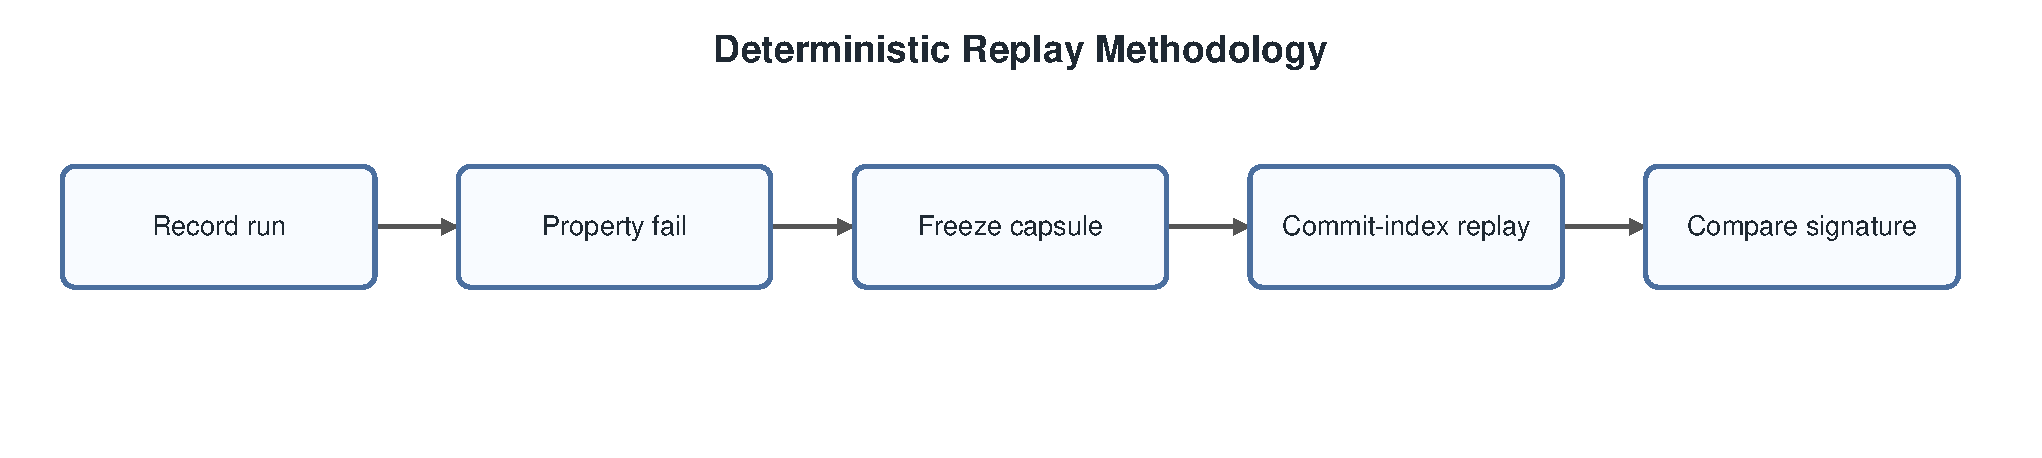
\includegraphics[width=\linewidth]{figures/replay_flow.pdf}}{\fbox{\parbox{0.9\linewidth}{Generated source: \texttt{paper/figures/replay\_flow.svg}}}}
\caption{Record/replay timeline with commit-indexed events. Source generated from \texttt{scripts/make\_figures.py}.}
\label{fig:timeline}
\end{figure}

The proof sketch in \texttt{formal/replay\_sufficiency\_theorem.md} is by induction over commit index: equal initial state, deterministic ordinary steps, equal boundary-event payloads at nondeterministic steps, and deterministic property checking over the equal prefix.

\section{Hardware Architecture}

ReplayCapsule-RV instruments the processor boundary rather than replacing the core. The PicoRV32 wrapper exposes memory, MMIO, interrupt, and commit-context signals to the record-side modules. The event tap observes candidate facts, the classifier selects replay-relevant and diagnostic classes, the slicer retains context around a property failure, the capsule buffer stores encoded packets, and the property checker freezes the capsule on a target violation.

\begin{figure}[t]
\centering
\IfFileExists{figures/architecture_overview.pdf}{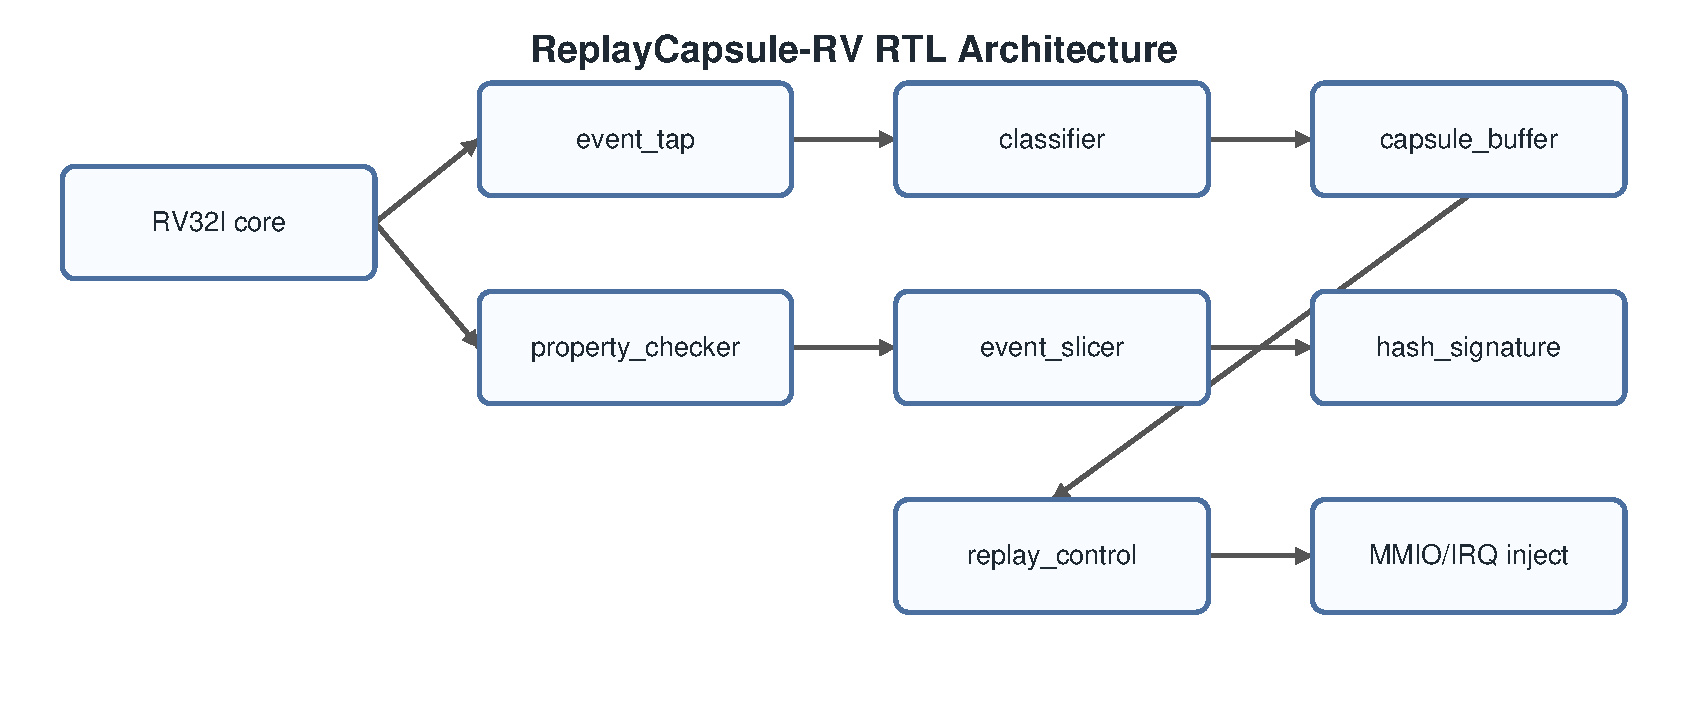
\includegraphics[width=\linewidth]{figures/architecture_overview.pdf}}{\fbox{\parbox{\linewidth}{Generated source: \texttt{paper/figures/architecture\_overview.svg}}}}
\caption{ReplayCapsule hardware architecture. Source generated from \texttt{scripts/make\_figures.py}.}
\label{fig:architecture}
\end{figure}

The board-level mapped wrappers expose only clock, reset, UART, GPIO, status LEDs, and three recorder-status pins. Large debug and internal buses remain inside the FPGA design. The prototype prioritizes replay fidelity and auditability over area minimization; Section~\ref{sec:evaluation} reports the generated same-target ECP5 mapped overhead rather than presenting the recorder as an optimized implementation.

\section{Replay Engine and Verification}

The replay comparator consumes an expected capsule and an observed replay trace. A passing comparison requires matching property metadata, the required event classes at the selected commit or cycle index, exact payload equality for replay-driving events, and no extra replay-driving events. Negative tests corrupt metadata, remove events, duplicate events, shift indices, swap order tags, and perturb payloads. The same comparator is used for model fixtures and exported RTL-smoke capsules.

\begin{table}[t]
\caption{Evidence levels and gate status. Generated sources include \texttt{results/processed/replay\_experiments.csv}, \texttt{results/processed/rtl\_capsule\_exports.csv}, and \texttt{results/processed/full\_rtl\_replay.csv}.}
\label{tab:evidence}
\centering
\begin{tabular}{lll}
\toprule
Level & Current role & Status meaning \\
\midrule
Model & event-level executable replay fixtures & generated pass rows \\
Firmware-sim & RV32I interpreter replay fixtures & generated pass rows \\
RTL-smoke & wrapper runs and capsule export checks & generated pass rows \\
Full RTL & firmware-running record/replay suite & blocked rows \\
Mapped synthesis & FPGA or ASIC reports & unavailable rows \\
\bottomrule
\end{tabular}
\end{table}

Bounded local checks cover recorder and control contracts such as event classification, buffer behavior, property signatures, replay mismatch handling, register access, hash/signature update, and MMIO/interrupt logging. These checks support local RTL obligations; they are not a mechanized end-to-end processor theorem.

\section{Evaluation}
\label{sec:evaluation}

The evaluation is generated from repository scripts and processed CSVs; the paper-number audit rejects numeric claims that do not appear in generated evidence. The core full-RTL ledger reports \rcFullReplayPass/\rcFullReplayTotal\ compiler-backed record/replay PASS rows. The negative ledger rejects \rcNegativeReject\ replay-critical corruptions, reports \rcNegativeUnexpectedAccept\ unexpected accepts, and leaves \rcNegativeNA\ not-applicable rows for corruption classes outside the current commit-index harness.

\subsection{Replay, Scale, and Buffers}

Replay succeeds on the fixed compiler-backed suite in the full-RTL harness, but scaling is constrained by capsule capacity. The regenerated workload-scaling evidence reports 375/375 PASS rows with workload-aware v1 depths: 256 for smoke and short workloads, 1024 for medium, 4096 for long, and 16384 for stress. The buffer-sensitivity table shows replay success reaches 100.000000\% for each workload class at those selected depths, while the sticky overflow bit remains asserted on long-running fixed and no-failure rows that do not freeze at a property failure. The paper therefore treats buffer depth as a design parameter, not a hidden constant.

Capsule-size comparisons use the buffer depth required for the workload class under test. \texttt{capsule\_baseline\_summary.csv} reports median ReplayCapsule reductions versus the raw full-instruction-trace estimate of 59.52\% for smoke, 78.71\% for short, 83.18\% for medium, 64.86\% for long, and 22.84\% for stress. The same CSV includes a labeled \texttt{riscv\_etrace\_branch\_trace\_estimate} row; that estimate is smaller than ReplayCapsule-RV for these workloads, so the raw instruction-trace comparison is a weak baseline, not a state-of-the-art trace-compression claim.

The v2 evidence package adds compressed recorder configurations and two additional actuator/configuration firmware families. Those rows improve workload and benchmark coverage for the scoped model, but they do not turn the standalone replay-consume controller into an integrated full-core autonomous replay path.

\subsection{Cost and Mapping}

The mapped FPGA results are same-target bring-up/debug measurements. The board-level baseline and ReplayCapsule wrappers use the same \rcMappedTarget\ target and \rcMappedFlow\ flow. After gating unselected v2 recorder instances in v1 mapped builds, the representative mapped-scaling summary reports LUT overhead from 114.20\% to 221.23\%, FF overhead from 174.53\% to 646.43\%, BRAM overhead of 0.00\%, and Fmax change from -19.56\% to -9.98\%.

For the selected v2 minimal recorder profile, the same-target ECP5 measured row reports +8.26\% LUT, +3.77\% FF, +0.00\% BRAM, and -0.04\% Fmax. The core and hashed v2 rows remain diagnostic-rich comparison points, with +68.00\% and +67.69\% LUT overhead and +81.49\% FF overhead. These rows support the design direction that replay-critical boundary-event capture should be separated from optional on-chip diagnostics.

This overhead is acceptable only under the intended use case: temporary validation and post-failure replay instrumentation during hardware/software bring-up. It is not presented as a production always-on block. The current artifact does not include an ASIC or power flow; FPGA results should be read as feasibility and cost-shape evidence rather than signoff implementation data.

\ifrcfullartifactpaper
% Auto-generated by scripts/render_paper_tables.py from results/processed/*.csv.

\begin{table}[t]
\caption{Compiler-backed firmware benchmark suite. Source: \texttt{results/processed/firmware\_build.csv}.}
\label{tab:benchmarks}
\centering
\begin{tabular}{lll}
\toprule
Family & Variants & Failure mechanism \\
\midrule
Sensor threshold & failing, fixed, no\_failure\_edge & MMIO sensor threshold and deadline check \\
Interrupt race & failing, fixed & interrupt delivery inside a critical window \\
MMIO ordering & failing, fixed & unsafe command/output MMIO ordering \\
Stack corruption & failing, fixed & protected-store observation reaches checker \\
UART command & failing, fixed, no\_failure\_edge & unsafe UART command drives actuator write \\
Watchdog timeout & failing, fixed, no\_failure\_edge & missed heartbeat under long-running path \\
\bottomrule
\end{tabular}
\end{table}

\begin{table}[t]
\caption{Host-driven full RTL replay success. Source: \texttt{results/processed/full\_rtl\_replay.csv}.}
\label{tab:replay-success}
\centering
\begin{tabular}{lrrl}
\toprule
Evidence & Pass & Total & Firmware source \\
\midrule
Record/replay/signature match & 45 & 45 & compiler C \\
Compiler-backed rows & 45 & 45 & compiler C \\
\bottomrule
\end{tabular}
\end{table}

\begin{table}[t]
\caption{Full RTL corrupted-capsule behavior. Source: \texttt{results/processed/full\_rtl\_replay\_negative.csv}.}
\label{tab:negative}
\centering
\begin{tabular}{lr}
\toprule
Result & Rows \\
\midrule
REJECT & 10 \\
ACCEPT & 0 \\
NA & 2 \\
\bottomrule
\end{tabular}
\end{table}

\begin{table}[t]
\caption{Runtime and simulator-overhead summary. Source: \texttt{results/processed/runtime\_overhead\_summary.csv}. Simulator wall time is not a hardware timing claim.}
\label{tab:runtime}
\centering
\begin{tabular}{llrr}
\toprule
Config & Metric & Median & N \\
\midrule
baseline no recorder & sim wall time sec & 0.018194 & 45 \\
recorder present disabled & sim wall time sec & 0.024409 & 45 \\
recorder enabled & sim wall time sec & 0.024731 & 45 \\
recorder present disabled vs baseline no recorder & cycle overhead pct & 0.000000 & 45 \\
recorder enabled vs baseline no recorder & cycle overhead pct & 0.000000 & 45 \\
recorder enabled vs baseline no recorder & sim wall time overhead pct & 33.950000 & 45 \\
\bottomrule
\end{tabular}
\end{table}

\begin{table}[t]
\caption{Full-core mapped ECP5 overhead. Sources: \texttt{results/processed/mapped\_synthesis.csv} and \texttt{results/processed/mapped\_overhead.csv}.}
\label{tab:mapped-overhead}
\centering
\begin{tabular}{lrrrr}
\toprule
Design/metric & LUT & FF & BRAM & Fmax MHz \\
\midrule
Baseline board & 2814 & 883 & 6 & 63.47 \\
ReplayCapsule board & 6859 & 3901 & 6 & 50.70 \\
Overhead & 143.75\% & 341.79\% & 0.00\% & -20.12\% \\
\bottomrule
\end{tabular}
\end{table}

\begin{table}[t]
\caption{Scope and limitations.}
\label{tab:limitations}
\centering
\begin{tabular}{ll}
\toprule
Topic & Current scope \\
\midrule
Processor & single-hart RV32I/PicoRV32 \\
Nondeterminism & commit-indexed interrupt/MMIO boundary events \\
Replay engine & host-driven Verilator harness \\
Replay hardware & record-side recorder only; no replay-consume datapath \\
Memory system & no multicore, DMA, cache-coherence, or analog-device model \\
Optimization & fidelity and auditability prioritized over area minimization \\
\bottomrule
\end{tabular}
\end{table}

\fi

\section{Related Work}

RISC-V E-Trace, N-Trace, and external debug specifications target processor observability, control-flow reconstruction, and standardized debug transport~\cite{riscvTrace,riscvDebug}. ReplayCapsule-RV is complementary: it records commit-indexed replay-driving interrupt/MMIO events for a scoped single-hart RV32I failure class. It does not attempt to provide architectural trace coverage or debug interoperability.

Post-silicon trace compression reduces trace bandwidth and storage by exploiting structure in instruction or control-flow streams. ReplayCapsule-RV makes a different tradeoff. It records the boundary events needed by the replay harness, not a compressed representation of the full executed instruction stream.

Deterministic replay systems record nondeterministic inputs and ordering so an execution can be reconstructed~\cite{leblanc1987debugging,dunlap2002revirt}. ReplayCapsule-RV borrows that replay discipline but narrows the target to embedded interrupt/MMIO failures, uses commit-indexed hardware capsules, and evaluates a PicoRV32 RTL harness rather than an operating-system or virtual-machine replay substrate.

Runtime verification and assertion monitors detect violations close to the hardware/software boundary~\cite{runtimeVerification}. ReplayCapsule-RV uses property checking as the capsule trigger, but its contribution is the replay-driving event stream and the evidence that corrupted capsules fail comparison.

Embedded event logs are widely used to explain firmware failures after deployment. ReplayCapsule-RV differs by making event ordering architectural through commit indices and by validating the capsule through replay comparison instead of presenting the log only as diagnostic text.

FPGA/emulation debugging and checkpointing can capture broad hardware state and rerun workloads under controlled conditions. Snapshot and time-travel systems similarly preserve enough state to resume or inspect execution~\cite{king2005debugging}. ReplayCapsule-RV is narrower: it keeps the same initial state and firmware image, then records the boundary events needed for a selected failure prefix.

The implementation builds on PicoRV32, Verilator, Icarus Verilog, Yosys, nextpnr, and bounded formal tooling~\cite{picorv32,verilator,icarus,yosys,nextpnr,symbiyosys}. These tools support reproducibility; the claimed research object is the scoped capsule model, recorder, replay harness, and evidence package.

\section{Limitations}

The scope is single-hart RV32I firmware with deterministic core semantics, the same program image, the same initial architectural state, and modeled external events. The current theorem excludes multicore interleavings, DMA unless modeled, cache/coherence effects unless modeled, analog nondeterminism, and claims about undefined C behavior.

MMIO side effects are modeled only at the replay-visible boundary. Interrupts are injected at an architectural boundary. Replay consumes every required event exactly once; missing, duplicate, reordered, or corrupted events must fail comparison. Capsule overflow invalidates replay availability.

The strongest generated evidence today is compiler-backed firmware, host-driven full RTL replay, full RTL corrupted-capsule rejection, runtime summaries, bounded local formal checks, generic synthesis context, and same-target full-core ECP5 mapped evidence. The artifact does not claim ASIC area or power, multi-hart behavior, DMA behavior, cache-coherence behavior, or a hardware replay-consume datapath.

\section{Conclusion}

ReplayCapsule-RV explores event-sufficient replay for embedded RV32I failures whose decisive nondeterminism comes through interrupts and memory-mapped I/O. The current artifact shows that the model, firmware-sim path, RTL-smoke exports, host-driven RTL replay rows, corruption checks, bounded local checks, scoped tiny mapped rows, and generated baselines can be reproduced without inventing missing hardware results. The remaining stronger evidence level is blocked until compiler-backed firmware, true runtime-overhead baselines, full-core mapped resource/timing reports, and a paper PDF build are generated.


\clearpage
\phantomsection
\label{aspdac:references-start}
\bibliographystyle{ACM-Reference-Format}
\bibliography{references}

\end{document}
